% v2-acmsmall-sample.tex, dated March 6 2012
% This is a sample file for ACM small trim journals
%
% Compilation using 'acmsmall.cls' - version 1.3 (March 2012), Aptara Inc.
% (c) 2010 Association for Computing Machinery (ACM)
%
% Questions/Suggestions/Feedback should be addressed to => "acmtexsupport@aptaracorp.com".
% Users can also go through the FAQs available on the journal's submission webpage.
%
% Steps to compile: latex, bibtex, latex latex
%
% For tracking purposes => this is v1.3 - March 2012

%\documentclass[prodmode,acmcsur]{acmsmall} % Aptara syntax
\documentclass[format=acmsmall, review=false]{acmart}

% Package to generate and customize Algorithm as per ACM style
\usepackage[ruled]{algorithm2e} 
\renewcommand{\algorithmcfname}{ALGORITHM}
\SetAlFnt{\small}
\SetAlCapFnt{\small}
\SetAlCapNameFnt{\small}
\SetAlCapHSkip{0pt}
\IncMargin{-\parindent}

% Metadata Information
\acmJournal{CSUR}
\acmVolume{0}
\acmNumber{0}
\acmArticle{0}
\acmYear{2018}
\acmMonth{0}
\copyrightyear{2018}

\acmDOI{0000001.0000001}
\setcopyright{none}

% !TEX root = main.tex
%\usepackage{a4wide}
\usepackage{listings}
\usepackage{comment}
\usepackage{amsmath}
\usepackage{graphicx}
\usepackage{amssymb}
\usepackage{url}
\usepackage{hyperref}
\usepackage{float}
\usepackage{lipsum}
\usepackage{caption}
\usepackage{subcaption}
\usepackage{adjustbox}
\usepackage{framed}
\usepackage{multirow}
\usepackage{framed}
\usepackage{enumitem}
\usepackage{epigraph}
\usepackage{wasysym} % \brokenvert
\usepackage{wrapfig}

%\usepackage[usenames, dvipsnames]{xcolor} % for acmart

% commands
%\newcommand{\fullver}{}
\ifdefined\fullver
\newcommand{\iffullver}[2]{#1}
\else
\newcommand{\iffullver}[2]{#2}
\fi

%\usepackage{tikz}
%\newcommand*\circled[1]{\tikz[baseline=(char.base)]{
%            \node[shape=circle,draw,inner sep=2pt] (char) {#1};}}


\renewcommand{\epigraphsize}{\footnotesize}
\setlength{\epigraphwidth}{10cm}
%\renewcommand{\epigraphrule}{0pt}

\definecolor{shadecolor}{rgb}{0.92,0.92,0.92}

\hypersetup{
  colorlinks = true, % colours links instead of ugly boxes
  urlcolor = blue, %  colour for external hyperlinks
  linkcolor = black, % colour of internal links
  citecolor = black, % colour of citations
  pdftitle = {A Survey of Symbolic Execution Techniques},
  pdfauthor= {Roberto Baldoni, Emilio Coppa, Daniele Cono D'Elia, Camil Demetrescu, Irene Finocchi}
}	


\newcommand{\mytempedit}[1]{\ignorespaces#1}
\newcommand{\revedit}[1]{{\color{blue}#1}}


\setlength{\FrameSep}{2pt}
\newcommand{\myparagraph}[1]{\medskip\noindent{\bf\small #1.} }
\newcommand{\myparagraphnoperiod}[1]{\medskip\noindent{\bf\small #1} }

% EDIT TO ENABLE NOTES
\newcommand{\mynote}[1]{\ignorespaces} % TODO
%\newcommand{\mynote}[1]{\marginpar{\raggedleft{\fontfamily{pbk}\selectfont\scriptsize{\em #1}}}}

\newcommand{\stwoe}{\text{S\textsuperscript{2}E}}
\newcommand{\myinput}[1]{\ifdefined\internalrep \input{../#1} \else \input{#1} \fi}
%\newcommand{\boxedexample}[1]{\vspace{2mm}\noindent\fbox{\parbox{0.98\textwidth}{{\em Example.} #1}}}

\ifdefined\arxivver
\newcommand{\boxedexample}[1]{
\begin{shaded}
\noindent{\bf\small Example.} #1
\end{shaded}
}
\else
\newcommand{\boxedexample}[1]{
%\vspace{-2mm}
\begin{shaded*}
\noindent{\bf\small Example.} #1
\end{shaded*}
%\vspace{-2mm}
}
\fi




% Document starts
\begin{document}

% Page heads
%\markboth{R. Baldoni, E. Coppa, D. C. D'Elia, C. Demetrescu, and I. Finocchi}{A Survey of Symbolic Execution Techniques}

% Title portion
\title[A Survey of Symbolic Execution Techniques]{A Survey of Symbolic Execution Techniques}
\author{Roberto Baldoni}
\email{baldoni@diag.uniroma1.it}
\author{Emilio Coppa}
\email{coppa@diag.uniroma1.it}
\author{Daniele Cono D'Elia}
\email{delia@diag.uniroma1.it}
\author{Camil Demetrescu}
\email{demetres@diag.uniroma1.it}
\author{Irene Finocchi}
\email{finocchi@di.uniroma1.it}
\affiliation{
	\institution{Sapienza University of Rome}
}

\authorsaddresses{Author's addresses: R. Baldoni, E. Coppa, D.C. D'Elia, and C. Demetrescu, Department of Computer, Control, and Management Engineering, Sapienza University of Rome; I. Finocchi, Department of Computer Science, Sapienza University of Rome. E-mail addresses: \{baldoni, coppa, delia, demetrescu\}@diag.uniroma1.it, finocchi@di.uniroma1.it.}

\renewcommand{\shortauthors}{R. Baldoni et al.}

\maketitle

\renewcommand{\thesection}{\Alph{section}}
%\renewcommand\thefigure{\thesection.\arabic{figure}} 
\setcounter{figure}{11} % we have 11 figures in the main article
\setcounter{page}{38}
\renewcommand\thepage{\arabic{page}} 

{\large{\bf SUPPLEMENTARY MATERIAL}}

% !TEX root = main.tex

\section{Symbolic execution of binary code}

The importance of performing symbolic analysis of a program's properties on binary code is on the rise for a number of reasons. Binary code analysis is attractive as it reasons on code that will actually execute: not requiring source code significantly extends the applicability of such techniques (to, e.g., common off-the-shelf proprietary programs, firmwares for embedded systems, malicious software), and it gives the ground truth important for security applications whereas source code analysis may yield misleading results due to compiler errors and optimizations~\cite{BITBLAZE-ICISS08}. Also, the recent advances in runtimes for programs written in dynamic languages brought just-in-time compilation to the masses, taking over on interpreters used when no efficient source-to-binary translation of code was statically possible. 

Analyzing binary code is commonly seen as a challenging task due to its complexity and lack of a high-level semantics\mynote{[D] I'm omitting obfuscation, code packing, and encryption for now}. Modern architectures offer complex instruction sets: modeling each instruction can be difficult, especially in the presence of multiple side effects on processor flags to determine branch conditions. The second major challenge comes from the lack of the higher-level semantics present in source code, especially when no debugging information is available. Types are not explicitly encoded in binary code: even with register types, it is common to store values from one type and read them as another. Similar considerations can be made for array bounds as well. Also, control-flow graph information is not explicitly available, as control flow is performed through jump instructions at both inter- and intra-procedural level. The function abstraction at the binary level does not exist as we intend it at source-code level: functions can be separated in non-contiguous pieces, and code may also call in the middle of a code block generated for a source-level function.

In the remainder of this section we provide an overview of how symbolic executors can address some of the most significant challenges in the analysis of binary code.

\subsection{Lifting to an Intermediate Representation}
\missing

\begin{figure}[h!]
  \centering
  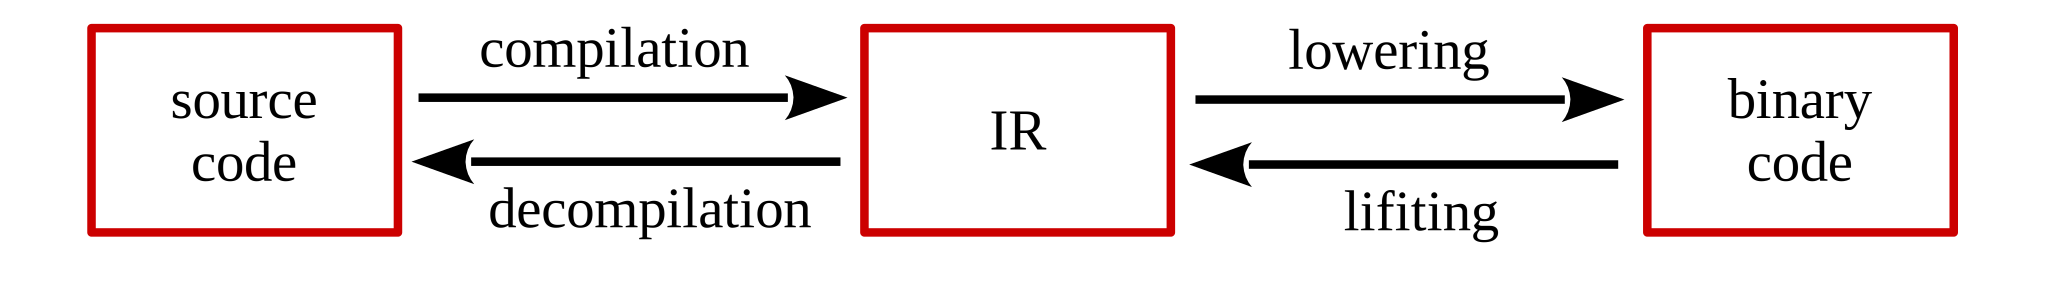
\includegraphics[width=.7\columnwidth]{images/compiler} 
\end{figure}

\vspace{2em}
\mynote{Notes from D\&E start here} For software such as common off-the-shelf programs, neither users nor attackers have access to their source code: 

Challenges (e.g., ~\cite{BITBLAZE-ICISS08}):
\begin{enumerate}
\item Complexity of the instruction sets
\item Lack of a higher-level semantics (functions/CFG, types, buffers)
\item Obfuscation/dynamic code generation
\end{enumerate}

Symbolic techniques may work on the source code or on the binary code. However, it is not uncommon that both the former and the latter work by reasoning on an intermediate representation of the original code. For instance, ~\cite{KLEE-OSDI08} interprets the LLVM bytecode generated by compiling the source code, while~\cite{ANGR-SP16} reasons on the VEX IR that has been obtained by lifting the binary code.


% !TEX root = appendix.tex

\section{Additional Tables}

\begin{table}[b]
  \centering
  %\begin{adjustbox}{width=\columnwidth}
  \begin{small}
  \begin{tabular}{| l || c || l |}
    \hline      
    {\bf Symbolic engine} & {\bf References} & {\bf Project URL} (last retrieved: December 2017)  \\ \hline\hline
    
    % CNC is not a symbolic engine but it uses constrained solver
    %{\sc Check 'n' Crash} & \cite{CS-ICSE05} & \url{http://ranger.uta.edu/~csallner/cnc/}\\
    
    {\sc CUTE} & \cite{CUTE-FSE05} & -- \\
    {\sc DART} & \cite{DART-PLDI05} & -- \\
    {\sc jCUTE} & \cite{SA-CAV06} & \url{https://github.com/osl/jcute} \\ % : Java Concolic Unit Testing Engine
    {\sc KLEE} & \cite{EXE-CCS06,KLEE-OSDI08} & \url{https://klee.github.io/} \\ % : a LLVM Execution Engine
    {\sc SAGE} & \cite{SAGE-NDSS08,EGL-ISSTA09} & -- \\
    {\sc BitBlaze} & \cite{BITBLAZE-ICISS08} & \url{http://bitblaze.cs.berkeley.edu/} \\ % , BHK-TR07
    {\sc CREST} & \cite{CREST-ASE08} & \url{https://github.com/jburnim/crest} \\ % : a concolic test generation tool for C
    {\sc PEX} & \cite{PEX-TAP08} & \url{http://research.microsoft.com/en-us/projects/pex/} \\
    {\sc Rubyx} & \cite{CF-CCS10} & -- \\
    {\sc Java PathFinder} & \cite{PATHFINDER-ASE10} & \url{http://babelfish.arc.nasa.gov/trac/jpf}\\
    {\sc Otter} & \cite{RSM-ICSE10} & \url{https://bitbucket.org/khooyp/otter/} \\
    {\sc BAP} & \cite{BAP-CAV11} & \url{https://github.com/BinaryAnalysisPlatform/bap} \\
    {\sc Cloud9} & \cite{CLOUD9-EUROSYS11} & \url{http://cloud9.epfl.ch/} \\
    {\sc Mayhem} & \cite{MAYHEM-SP12} & -- \\
    {\sc SymDroid} & \cite{JMF-TECH12} & -- \\
    {\sc \stwoe} & \cite{CKC-TOCS12} & \url{http://s2e.systems/} \\
    {\sc FuzzBALL} & \cite{MMP-ASPLOS12,FUZZBALL-ESORICS13} & \url{http://bitblaze.cs.berkeley.edu/fuzzball.html} \\
    {\sc Jalangi} & \cite{SKB-FSE13} & \url{https://github.com/Samsung/jalangi2} \\
    {\sc Pathgrind} & \cite{S-ICSE04} & \url{https://github.com/codelion/pathgrind} \\
    {\sc Kite} & \cite{V-THESIS14} & \url{http://www.cs.ubc.ca/labs/isd/Projects/Kite} \\
    {\sc SymJS} & \cite{LAG-FSE14} & -- \\
    {\sc CIVL} & \cite{CIVL-SC15} & \url{http://vsl.cis.udel.edu/civl/}\\ % : The Concurrency Intermediate Verification Language 
    {\sc KeY} & \cite{HBR-RV14} & \url{http://www.key-project.org/} \\
    {\sc Angr} & \cite{FIRMALICE-NDSS15,ANGR-SSP16} & \url{http://angr.io/} \\
    {\sc Triton} & \cite{TRITON-SSTIC15} & \url{http://triton.quarkslab.com/} \\
    {\sc PyExZ3} & \cite{BD-TECH15} & \url{https://github.com/thomasjball/PyExZ3} \\
    {\sc JDart} & \cite{JDART-TACAS16} & \url{https://github.com/psycopaths/jdart} \\

    {\sc CATG} & -- & \url{https://github.com/ksen007/janala2} \\
    {\sc PySymEmu} & -- & \url{https://github.com/feliam/pysymemu/} \\
    {\sc Miasm} & -- & \url{https://github.com/cea-sec/miasm} \\
    
    \hline  
  \end{tabular}
  \end{small}
  %\end{adjustbox}
  \caption{Selection of symbolic execution engines, along with their reference article(s) and software project web site (if any).}
  \label{tab:symbolic-engines}
  \vspace{-3.2mm} % TODO
\end{table}

\vspace{-2pt}
\myparagraph{Tools}
Table~\ref{tab:symbolic-engines} lists a number of symbolic execution engines that have worked as incubators for several of the techniques surveyed in this article. The novel contributions introduced by tools that represented milestones in the area are described in the appropriate sections throughout the main article.

\vspace{-1pt}
\myparagraph{Path Selection Heuristics}
Table~\ref{tab:heuristics} provides a categorization of the search heuristics that have been discussed in Section 2.3 of the main article. For each category, we list several works that have proposed interesting embodiments of the category.

\begin{table}[t]
  \centering
  \begin{adjustbox}{width=0.95\linewidth} % TODO was 1; with 0.88 the last paragraph will fit
  \begin{small}
  \begin{tabular}{| l || l |}
    \hline      
    {\bf Heuristic} & {\bf Goal} \\ \hline\hline
    BFS & {\em Maximize coverage} \cite{CKC-TOCS12,PEX-TAP08} \\ \hline
    DFS & {\em Exhaust paths, minimize memory usage} \cite{EXE-CCS06,CKC-TOCS12,PEX-TAP08,DART-PLDI05} \\\hline
    Random path selection & {\em Randomly pick a path with probability based on its length} \cite{KLEE-OSDI08} \\\hline
    %low-covered code & prioritize paths that execute low-covered code  & \cite{EXE-CCS06} \\
    \multirow{2}*{Code coverage search} & {\em Prioritize paths that may explore unexplored code or that may soon} \\ & {\em reach a particular target program point}  \cite{EXE-CCS06,KLEE-OSDI08,MAYHEM-SP12,CKC-TOCS12,GV-ISSTA02,MPF-SAS11} \\\hline
    Buggy-path-first & {\em Prioritize bug-friendly path} \cite{AEG-NDSS11} \\\hline
    Loop exhaustion & {\em Fully explore specific loops} \cite{AEG-NDSS11} \\\hline
    Symbolic instruction pointers & {\em Prioritize paths with symbolic instruction pointers} \cite{MAYHEM-SP12} \\\hline
    Symbolic memory accesses & {\em Prioritize paths with symbolic memory accesses} \cite{MAYHEM-SP12} \\ \hline
    Fitness function & {\em Prioritize paths based on a fitness function} \cite{XTD-DSN09,CS-CACM13,XTD-DSN09} \\ \hline
    \multirow{2}*{Subpath-guided search} & {\em Use frequency distributions of explored subpaths to prioritize less covered}\\ & {\em parts of a program} \cite{LZL-OOPSLA13} \\ \hline
    Property-guided search & {\em Prioritize paths that are most likely to satisfy the target property} \cite{ZCWDL15} \\ 
    %kill path & filter uninteresting path & \cite{CKC-TOCS12} \\
    \hline  
  \end{tabular}
  \end{small}
  \end{adjustbox}
  \caption{Common path selection heuristics discussed in Section 2.3.} % of the main article
  \label{tab:heuristics}
\end{table}

% !TEX root = appendix.tex

\section{Sample Applications}
\label{se:applications}

%\revedit{
The last decade has witnessed an increasing adoption of symbolic execution techniques not only in the software testing domain, but also to address other compelling engineering problems such as automatic generation of exploits or authentication bypass. We now discuss \iffullver{three prominent}{prominent} applications of symbolic execution techniques to these domains. Examples of extensions to other areas can be found, e.g., in~\cite{CGK-ICSE11}.
%}

%The last decade has witnessed an increasing adoption of symbolic execution techniques not only in the software testing domain, but also to address other compelling engineering problems such as automatic generation of exploits or authentication bypass. We now discuss \iffullver{three prominent}{prominent} applications of symbolic execution techniques to these domains. Examples of extensions to other areas can be found, e.g., in~\cite{CGK-ICSE11}.

\subsection{Bug Detection}\mynote{Rendere piu' di ampio respiro il titolo di questa sezione? Keyword: software testing, program understanding}
\label{ss:bug-detection}

Software testing strategies typically attempt to execute a program with the intent of finding bugs. As manual test input generation is an error-prone and usually non-exhaustive process, automated testing technique have drawn a lot of attention over the years. Random testing techniques such as fuzzing are cheap in terms of run-time overhead, but fail to obtain a wide exploration of a program state space. Symbolic and concolic execution techniques on the other hand achieve a more exhaustive exploration, but they become expensive as the length of the execution grows: for this reason, they usually reveal shallow bugs only.

\cite{RK-ICSE07} proposes {\em hybrid concolic testing} for test input generation, which combines random search and concolic execution to achieve both deep program states and wide exploration. The two techniques are interleaved: in particular, when random testing saturates (i.e., it is unable to hit new code coverage points after a number of steps), concolic execution is used to mutate the current program state by performing a bounded depth-first search for an uncovered coverage point. For a fixed time budget, the technique outperforms both random and concolic testing in terms of branch coverage. The intuition behind this approach is that many programs show behaviors where a state can be easily reached through random testing, but then a precise sequence of events -- identifiable by a symbolic engine -- is required to hit a specific coverage point.

% which uses preconstraining on the program states to ensure consistency
\cite{DRILLER-NDSS16} refines this idea and devises a vulnerability excavation tool based on {\sc Angr}~\cite{ANGR-SSP16}, called Driller, that interleaves fuzzing and concolic execution to discover memory corruption vulnerabilities. The authors remark that user inputs can be categorized as {\em general} input, which has a wide range of valid values, and {\em specific} input: a check for particular values of a specific input then splits an application into {\em compartments}. Driller offloads the majority of unique path discovery to a fuzzy engine, and relies on concolic execution to move across compartments. During the fuzzy phase, Driller marks a number of inputs as interesting (for instance, when an input was the first to trigger some state transition) and once it gets stuck in the exploration, it passes the set of such paths to a concolic engine, which preconstraints the program states to ensure consistency with the results of the native execution. On the dataset used for the DARPA Cyber Grand Challenge qualifying event, Driller could identify crashing inputs in 77 applications, including both the 68 and 16 applications for which fuzzing and symbolic execution alone succeeded, respectively. For 6 applications, Driller was the only one to detect a vulnerability.

% temporaneamente messo qui
\mytempedit{
	Maintenance of large and complex applications is a very hard task. Fixing bugs can sometimes even introduce new and unexpected issues in the software, which in turn may require several hours or even weeks to be detected and properly addressed by the developers. \cite{QRL-TOSEM12} tackles the problem of identifying the root cause of failures during regression testing. Given a program $P$ and a newer revision of the program $P'$, if a testing input $t$ generates a failure in $P'$ but not in  $P$, then symbolic execution is used to track the path constraints $\pi$ and $\pi'$ when executing $P$ and $P'$ on the failing input $t$, respectively. Using a SMT solver, a new input $t'$ is generated by solving the constraint $\pi ~\wedge \neg\pi'$. If $t'$ exists (i.e., the constraint is satisfiable), then $P'$ has one or more {\em deviations} in the control-flow graph with respect to $P$ that can be the root cause of the failure. By carefully tracking branch conditions during symbolic execution, \cite{QRL-TOSEM12} are even able to pinpoint which branches are responsible for these deviations. If $\pi \wedge \neg\pi'$ is not satisfiable, then the symmetric constraint query $\neg\pi \wedge \pi'$ is tested and a similar reasoning is performed to detect the possible branch conditions that may have lad to the failure. If $\neg\pi \wedge \pi'$ is also unsatisfiable, then \cite{QRL-TOSEM12} cannot determine the root cause of the problem.

	Another interesting work that targets the problem of software regressions through the use of symbolic execution is~\cite{BOR-ICSE13}. This work introduce an approach called {\em partition-based regression verification} that combines the advantages of both regression verification (RV) and regression testing (RT). Indeed, RV is a very powerful technique for identifying regressions but hardly scales over large programs due to the difficulty in proving behavioral equivalence between the original and the modified program. On the other hand, RT allows to check a modified program for regressions by testing selected concrete sample inputs, making it more scalable but providing limited verification guarantees. The main intuition behind partition-based regression verification is to identify {\em differential partitions}. Each differential partition can be seen as a subset of the input space for which the two program versions -- given the same path constraints -- either expose the same output ({\em equivalence-revealing partition}) or produce different outputs ({\em difference-revealing partition}). For each partition, a test case is generated and added to the regression test suite, which can later be used by a developer for classical RT. Since differential partitions are derived exploiting symbolic execution, this approach suffers from the common limitations that come with this technique. However, if the exploration is interrupted (e.g., due to excessive time or memory usage), partition-based regression verification can still provide guarantees over the subset of input space that has been covered by the detected partitions.

	Static data flow analysis tools can significantly help developers tracks malicious data leaks in software applications. Unfortunately, they often report several allegedly bugs that only after manual inspection can be regarded as false positives. To mitigate this issue,~\cite{ARH-SOAP15} has proposed TASMAN, a system that, after performing data flow analysis to track information leaks, uses symbolic backward execution (SBE) to test each reported bug. Starting from a leaking statement, TASMAN backwards into the code, pruning any path that can be proved to be unfeasible. If all the paths starting from the leaking statement are discarded by TASMAN, then the reported bug can be marked as a false positive.

	Although symbolic execution has been extensively used for bug detection, during the last decades several works~\cite{GDV-ISSTA12,FPV-ICSE13,CLL-ICSE16} have shown how it can be also used for other program understanding activities. For instance,~\cite{GDV-ISSTA12} has introduced {\em probabilistic symbolic execution}, an approach that makes it possible to compute the probability of executing different code portions of a program. This is achieved by exploiting model counting techniques, such as the {\tt LattE}~\cite{LHT-JSC04} toolset, that allows~\cite{GDV-ISSTA12}  to determine the number of solutions for the different path constraints given by the alternative execution paths of a program. The paper by~\cite{FPV-ICSE13} makes a step further and uses probabilistic symbolic execution for performing software reliability analysis. This is computed as the probability of executing any path that has been labeled as successful given a usage profile. Intuitively, a usage profile can be seen as the distribution over the input space. Since in general the termination of symbolic execution cannot be guaranteed in presence of loops, then~\cite{FPV-ICSE13} resorts to bounded exploration. Nonetheless, they define a metric for evaluating the confidence in their reliability estimation, allowing a developer to increase the bounds in order to improve the confidence value. Of a different flavor is the work by~\cite{CLL-ICSE16} that exploits probabilistic symbolic execution to conduct performance analysis. Based on usage profiles and on path execution probabilities, paths are classified into two types: {\em low probability} and {\em high probability}. In a first phase, high-probability paths are explored in a way that maximizes path diversity, generating a first set of test inputs. In the second phase, low-probability paths are analyzed using symbolic execution, generating a second set of test inputs that should expose executions characterized by best-execution times and by worst-execution times. Finally, the program is executed using the test inputs generated during the two phases and running times are measured to generate performance distributions. 

	Another interesting application of symbolic execution is presented by~\cite{PPM-CSF18}. Their technique exploits model counting and symbolic execution for computing quantitative bounds on the amount of information that can be leaked by a program through side-channel attacks. 
	
}
%As it is based on {\sc Angr}, Driller adopts an index-based memory model as in Section~\ref{ss:index-based-memory} where reads can be symbolic and writes are always concretized. % read/write addresses

\subsection{Bug Exploitation}
\label{ss:bug-exploitation}
Bugs are a consequence of the nature of human factors in software development and are everywhere. Those that can be exploited by an attacker should normally be fixed first: systems for automatically and effectively identifying them are thus very valuable.

{\sc AEG}~\cite{AEG-NDSS11} employs preconditioned symbolic execution to analyze a potentially buggy program in source form and look for bugs amenable to stack smashing or return-into-libc exploits~\cite{PB-SSP04}, which are popular control hijack attack techniques. The tool augments path constraints with exploitability constraints and queries a constraint solver, generating a concrete exploit when the constraints are satisfiable. The authors devise the {\em buggy-path-first} and {\em loop-exhaustion} strategies (Table~\ref{tab:heuristics}) to prioritize paths in the search. On a suite of 14 Linux applications, {\sc AEG} discovered 16 vulnerabilities, 2 of which were previously unknown, and constructed control hijack exploits for them.

{\sc Mayhem}~\cite{MAYHEM-SP12} takes another step forward by presenting the first system for binary programs that is able identify end-to-end exploitable bugs. It adopts a hybrid execution model based on checkpoints and two components: a concrete executor that injects taint-analysis instrumentation in the code and a symbolic executor that takes over when a tainted branch or jump instruction is met. Exploitability constraints for symbolic instruction pointers and format strings are generated, targeting a wide range of exploits, e.g., SEH-based and jump-to-register ones. Three path selection heuristics help prioritizing paths that are most likely to contain vulnerabilities (e.g., those containing symbolic memory accesses or instruction pointers). A virtualization layer intercepts and emulates all the system calls to the host OS, while preconditioned symbolic execution can be used to reduce the size of the search space. Also, restricting symbolic execution to tainted basic blocks only gives very good speedups in this setting, as in the reported experiments more than $95\%$ of the processed instructions were not tainted. {\sc Mayhem} was able to find exploitable vulnerabilities in the 29 Linux and Windows applications considered in the evaluation, 2 of which were previously undocumented. Although the goal in {\sc Mayhem} is to reveal exploitable bugs, the generated simple exploits can be likely transformed in an automated fashion to work in the presence of classical OS defenses such as data execution prevention and address space layout randomization~\cite{Q-SEC11}. 

\vspace{-1mm} % TODO
\subsection{Authentication Bypass}
\label{ss:auth-bypass}
Software backdoors are a method of bypassing authentication in an algorithm, a software product, or even in a full computer system. Although sometimes these software flaws are injected by external attackers using subtle tricks such as compiler tampering~\cite{KRS-TR74}, there are reported cases of backdoors that have been surreptitiously installed by the hardware and/or software manufacturers~\cite{CZF-USEC14}, or even by governments~\cite{NSA-BACKDOOR}. 

Different works~\cite{DMR-USEC13,ZBF-NDSS14,FIRMALICE-NDSS15} have exploited symbolic execution for analyzing the behavior of binary firmwares. Indeed, an advantage of this technique is that it can be used even in environments, such as embedded systems, where the documentation and the source code that are publicly released by the manufacturer are typically very limited or none at all. For instance,~\cite{FIRMALICE-NDSS15} proposes Firmalice, a binary analysis framework based on {\sc Angr}~\cite{ANGR-SSP16} that can be effectively used for identifying authentication bypass flaws inside firmwares running on devices such as routers and printers. Given a user-provided description of a privileged operation in the device, Firmalice identifies a set of program points that, if executed, forces the privileged operation to be performed. The program slice that involves the privileged program points is then symbolically analyzed using {\sc Angr}. If any such point can be reached by the engine, a set of concrete inputs is generated using an SMT solver. These values can be then used to effectively bypass authentication inside the device. On three commercially available devices, Firmalice could detect vulnerabilities in two of them, and determine that a backdoor in the third firmware is not remotely exploitable.

% Bibliography
%\bibliographystyle{abstract} 
\bibliographystyle{ACM-Reference-Format}
\bibliography{symbolic}

% History dates
%\received{--- 2016}{--- XXXX}{---- XXXX}

\end{document}

% End of v2-acmsmall-sample.tex (March 2012) - Gerry Murray, ACM


